\documentclass{standalone}
\usepackage{tikz}
\usepackage{ctex,siunitx}
\usepackage{tkz-euclide}
\usepackage{amsmath}
\usetikzlibrary{patterns, calc}
\usetikzlibrary {decorations.pathmorphing, decorations.pathreplacing, decorations.shapes,}
\begin{document}
\small
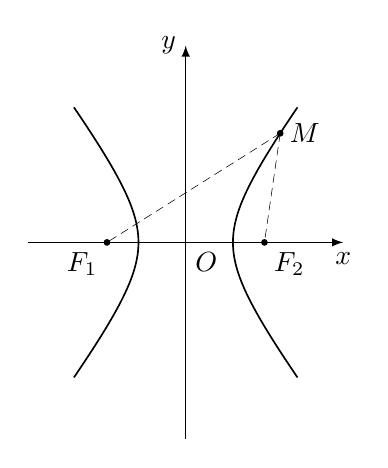
\begin{tikzpicture}[>=latex,scale=1]
  \draw[thin,->](-2,0)--(2,0)node[below]{$x$};
  \draw[thin,->](0,-2.5)--(0,2.5)node[left]{$y$};
  \tkzDefPoints{0/0/O,-1/0/F1,1/0/F2}
  \draw[semithick,domain=-65:65,samples=200] plot ({0.6/cos(\x)},{0.8*tan(\x)});
  \draw[semithick,domain=-65:65,samples=200] plot ({-0.6/cos(\x)},{0.8*tan(\x)});
  \tkzDefPoint(1.2,{0.8*sqrt(3)}){M}
  \tkzDrawSegments[densely dashed](M,F1 M,F2)
  \tkzDrawPoints[fill=black](F1,F2,M)
  \tkzLabelPoints[right](M)
  \tkzLabelPoint[below left](F1){$F_1$}
  \tkzLabelPoint[below right](F2){$F_2$}
  \tkzLabelPoints[below right](O)
\end{tikzpicture}
\end{document}